\section{Scope of Work}

\subsection{Initial Situation}
With shaders making up a large part of visual effects in games and in game development generally, they have become more and more important throughout the years. Due to their high flexibility, it is possible to create a wide variation of implementations as well as cheap alternatives to otherwise highly complex and computationally demanding simulations, such as simulating water, fire or clouds.
\\ This project specifically focuses on clouds. But to achieve a realistic look and feel of the clouds, certain methods and knowledge are required. The motivation for this project is to implement such a shader based on information gathered during the given period.


\subsection{Goals}
The primary goal of the project is to research and document rendering techniques for real-time procedural cloud shaders. Additionally, a prototype is to be implemented based on the newly discovered knowledge.

\subsubsection{Mandatory Goals}
The following tasks must be accomplished during the project:
\begin{itemize}
\item Understanding of the basic nature of clouds
\item Understanding of what makes good clouds in games
\item Research common methods and algorithms involved in rendering procedural clouds, including...
    \begin{itemize}
    \item volumetric rendering
    \item procedural noise generation algorithms
    \item the concept of ray-marching
    \end{itemize}
\end{itemize}

\subsubsection{Optional Goals}
For further optional research, these tasks can be looked into:
\begin{itemize}
    \item Light scattering illumination and sub-surface scattering
    \item Performance optimization
    \item Simulation of gas
\end{itemize}

\clearpage

\subsection{Vision}
asdads

\begin{figure}[ht]
    \centering
    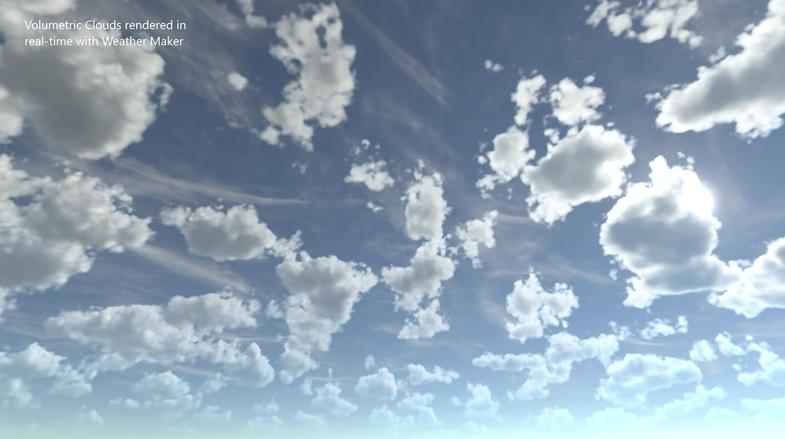
\includegraphics[width=0.45\linewidth]{rendered-clouds-02}
    \hspace{0.02\linewidth}
    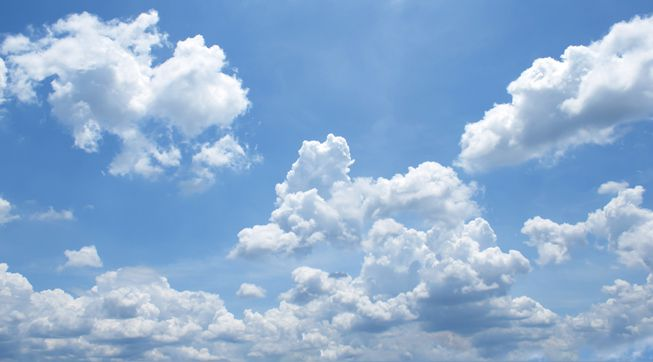
\includegraphics[width=0.45\linewidth]{photographic-clouds-01}
    \caption{A rendered image of volumetric clouds\protect\cite{img:rendered:clouds02} (left) and a photographic reference of clouds\protect\cite{img:photo:clouds01} (right). }
    \label{fig:vision} 
\end{figure}

\subsection{Educational Objectives}
Educational objectives include shader programming, rendering techniques, common algorithms used in computer graphics, a general understanding about the role of clouds in games and other topics.

\subsection{Used software}
All documentation will be made in Visual Studio Code.
The shader will be implemented in Unity. The chosen language is \gls{hlsl}.